\subsection{Aire Guru}
Practical - show by example (Aire Guru)
Datos de origen
Aire Guru utiliza los datos de calidad del aire proporcionados por el ayuntamiento de Malaga en su portal de datos abiertos.
\begin{figure}[h]
    \centering
    \includegraphics[width=8cm]{OpenDataPortal}
    \caption{Open Data Portal Malaga}
    \end{figure}

Los datos extraidos estan en formato GeoJSON, este formato proporciona un documento JSON con subdocumentos anidados, cada uno de estos
subdocumentos contiene un conjunto de datos en forma clave valor. 

En la siguiente figura podemos ver el principio del documento descargado el 09 de Junio del 2019 
\footnote{\url{https://datosabiertos.malaga.eu/recursos/ambiente/calidadaire/calidadaire.json}}
En este extracto podemos ver los primeros dos subdocumentos.. Un subdocumento contiene las coordenadas de la estacion medidora de la calidad
del aire, la fecha y hora cuando se tomo y a continuacion los valores de las mediciones. En la figura siguiente podemos encontrar la descripcion
proporcionada por el portal de datos abiertos.
\begin{figure}[ht]
    \centering
    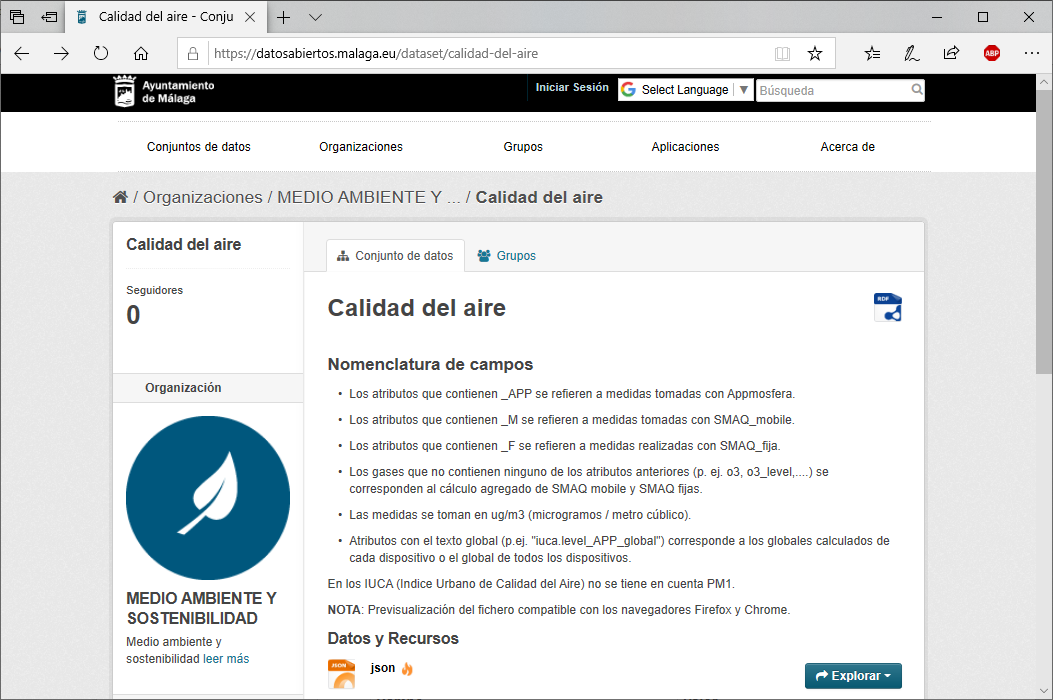
\includegraphics[width=8cm]{geoJsonAirQualityDataDescription}
    \caption{Air quality data description [09/06/2019].Open Data Portal Malaga}
\end{figure}

\begin{figure}[ht]
    \centering
    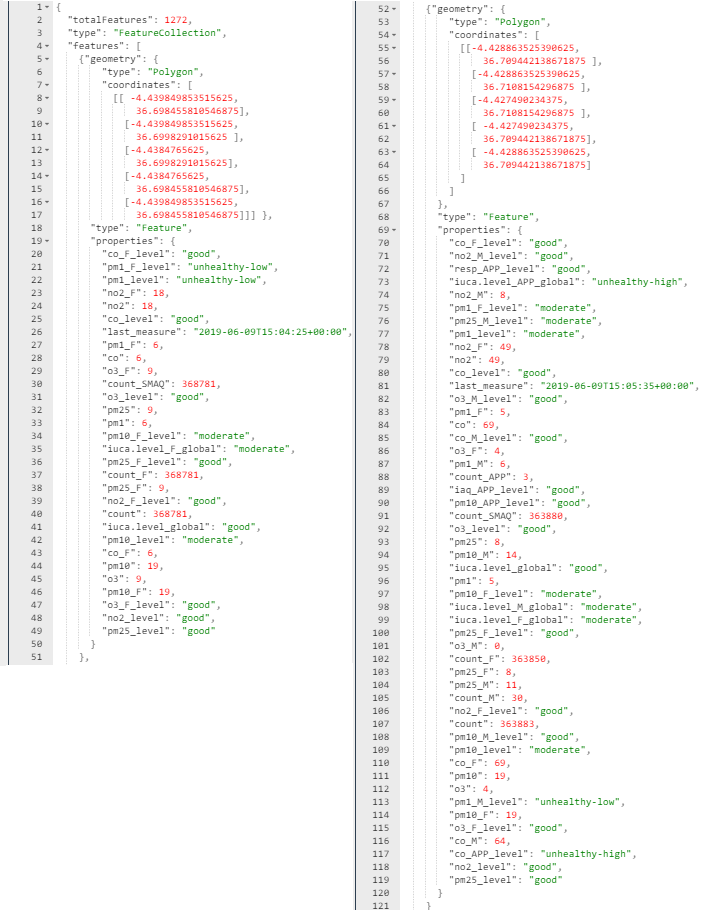
\includegraphics[width=8cm]{geoJsonAirQualityData}
    \caption{Air quality Document [09/06/2019].Open Data Portal Malaga}
    \end{figure}

    Podemos comprobar que el segundo de ellos ha registrado un numero distintos de
    campos.




    
   


La herramienta Aire guru presenta la informacion en el idioma nativo de la ciudad y actualmente se esta trabajando en su traduccion 
al ingles, para cubrir un rango mas amplio de su poblacion, ya que esta ciudad es cada vez mas cosmopolita.
Se utiliza un lenguaje sencillo y directo y se acompana de pictogramas, facil de identificar, para una
lectura mas rapida de la situacion.



--acceso a los datos
Aire Guru esta disponible al usuario mediante la url segura https://www.aire.guru y https://www.airquality.guru.
El uso de SSL proporciona ademas de 
--navegadores
una opcion segura para los usuarias, ya que asegura en envio de informacion a traves de la red de forma
cifrada.
Para acceder a la informacion general
--lectura familiar de los datos
iconografia
colores oficiales
